\documentclass[11pt,a4paper]{article}
\usepackage{{../../paquete-formulas}}
\usepackage{{../../estilos-formulas}}

\newcommand{\materia}{Electrónica Industrial}

\begin{document}
	\pagestyle{pieyencabezado}
	\section*{Nomenclatura}
	
	\begin{tabular}{r l r l}
		$V_Z$ & Tensión en el Zener & $I_Z$ & Corriente en el Zener\\
		$V_F$ & Tensión de la fuente & $I_L$ & Corriente en la carga\\
		$i_C$ & Corriente del colector & $v_{CE}$ & Tensión en juntura C E \\
		$i_B$ & Corriente de la base & $v_{CB}$ & Tensión en juntura C B \\
		$i_E$ & Corriente del emisor & $v_{BE}$ & Tensión en juntura B E \\
		$\beta$ & Ganancia en corriente & $\alpha$ & Parámetro alpha\\
		$V_{Th}$ & Tensión de Thévenin & $R_{Th}$ & Resistencia de Thévenin \\
		
	\end{tabular}
	\unidad{1}{Dispositivos de estado sólido}
	\begin{multicols}{2}
		
		\begin{cajita}
				\subtitulo{Diodos}
		\end{cajita}
		
		
		\begin{cajita}
			
			\subtitulo{Diodo Zener}
			
			\subsubtitulo{Estados del zener}
			
			\vspace{-.6cm}
			
			\begin{multicols}{2}
				\begin{tabular}{l l l}
					\multicolumn{3}{l}{Condiciones mínimas} \vspace{.1cm}\\
					${V_F}_{mín}$ & ${I_Z}_{mín}$ & ${I_L}_{máx}$\vspace{.1cm}\\
					\multicolumn{3}{l}{Condiciones máximas}\vspace{.1cm}\\
					${V_F}_{máx}$ & ${I_Z}_{máx}$ & ${I_L}_{mín}$
				\end{tabular}
			
				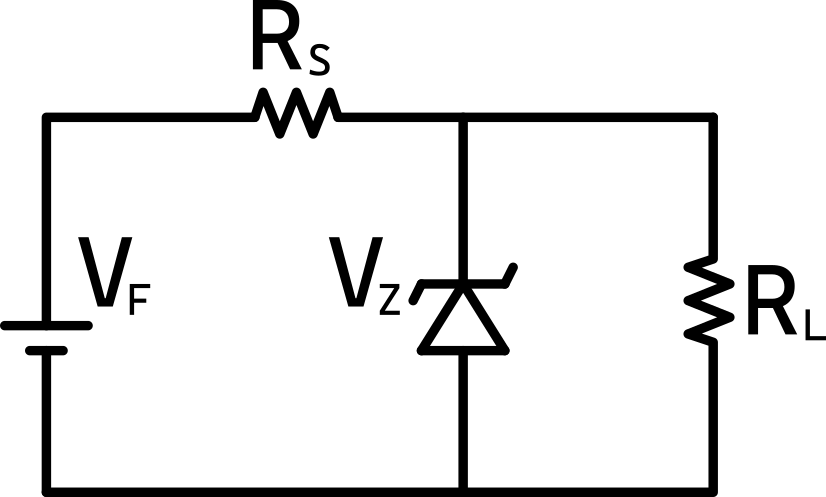
\includegraphics[width = .9\linewidth]{circuito-zener}
			\end{multicols}
			
		\end{cajita}
	
	\end{multicols}

	\unidad{2}{Transistores}
	
	
	\begin{multicols}{2}
		
		\begin{cajita}
			
			\subtitulo{Transistor bipolar BJT}
			\vspace{.5cm}
			\begin{tabular}{l l}
				Tensión en la juntura B E & $v_{BE} = 0,7 \textnormal{ V}$
			\end{tabular}
			\subsubtitulo{Tipo constructivo}\vspace{-.2cm}
			
			\begin{tabular}{c c}
				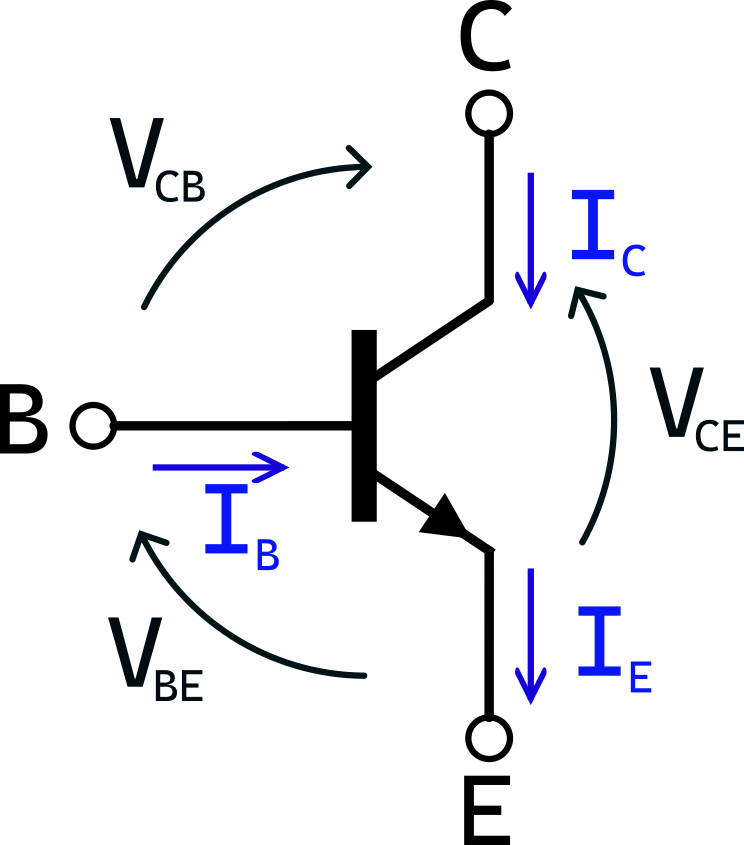
\includegraphics[width = .4\linewidth]{transistor-npn} & 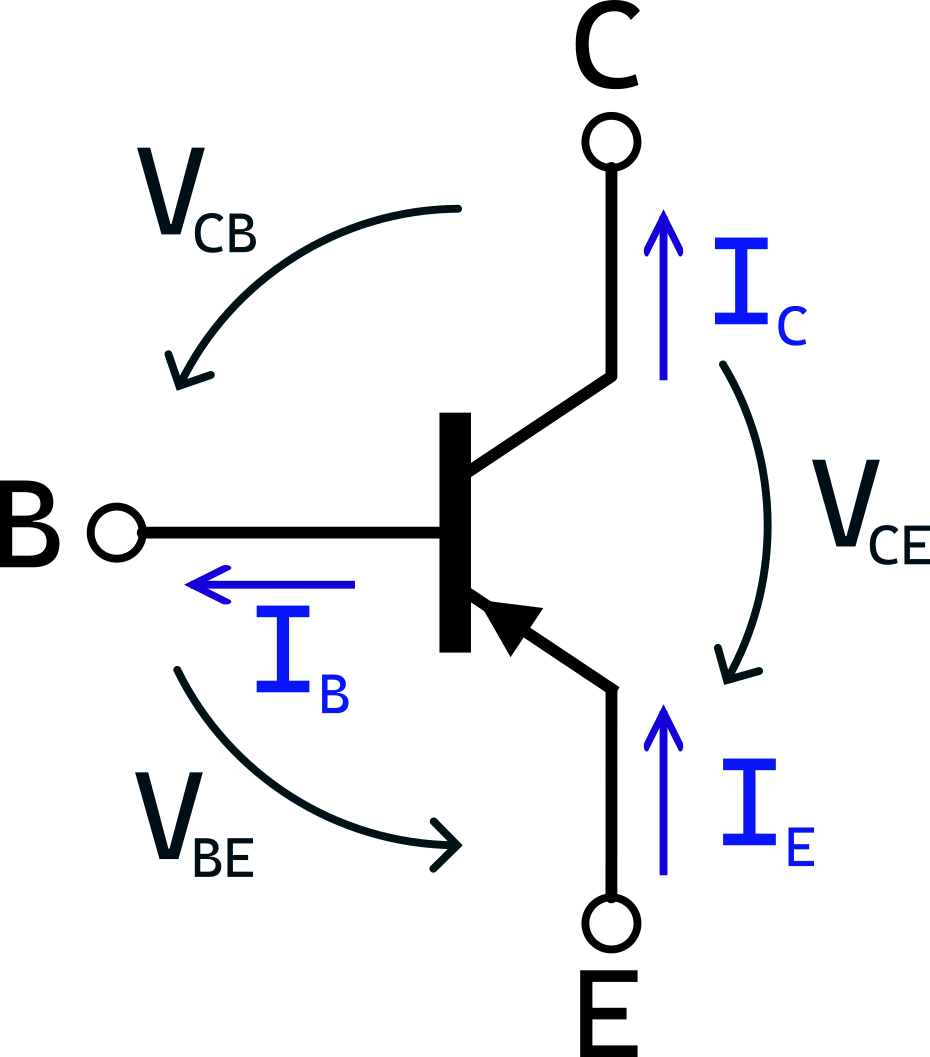
\includegraphics[width = .4\linewidth]{transistor-pnp} \\
				\textsc{npn} & \textsc{pnp} \\
				Ingresa corriente a E & Sale corriente de E
			\end{tabular}
			\subsubtitulo{Configuración}
			\begin{tabular}{c c c}
				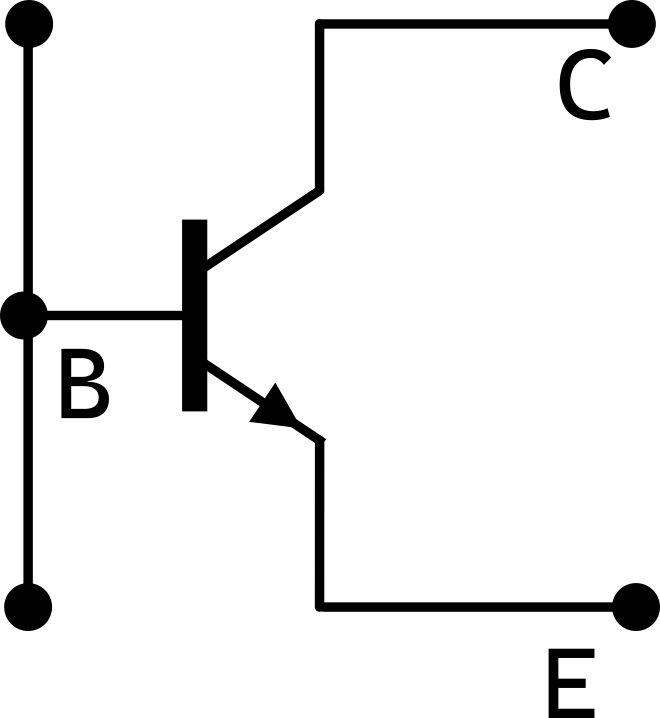
\includegraphics[width = .2\linewidth]{base-comun} & 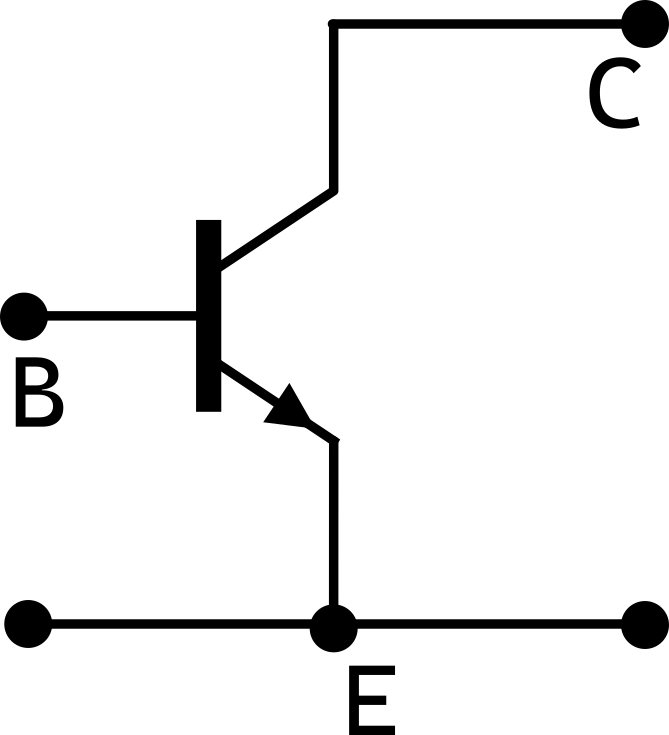
\includegraphics[width = .2\linewidth]{emisor-comun} & 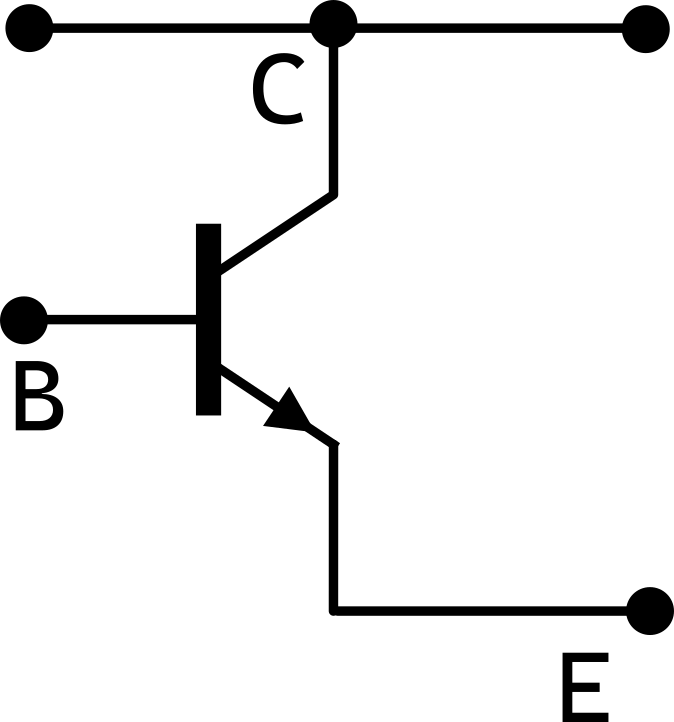
\includegraphics[width = .2\linewidth]{colector-comun} \\
				\textsl{Base común} & \textsl{Emisor común} & \textsl{Colector común}
			\end{tabular}
		\end{cajita}
	
	\columnbreak %Revisar después
	
		\begin{cajita}
			\subtitulo{Polarización del BJT}
			
			\subsubtitulo{Ecuaciones del dispositivo}\vspace{-.3cm}
					
			\begin{tabular}{l l}
				$i_C = \alpha i_E$ & Si no se especifica: $\alpha = 1 $ \\[.1cm]
				$i_C = \beta i_B$ & $i_E = i_B + i_C$ \\
			\end{tabular}
		
			\vspace{.2cm}
		
			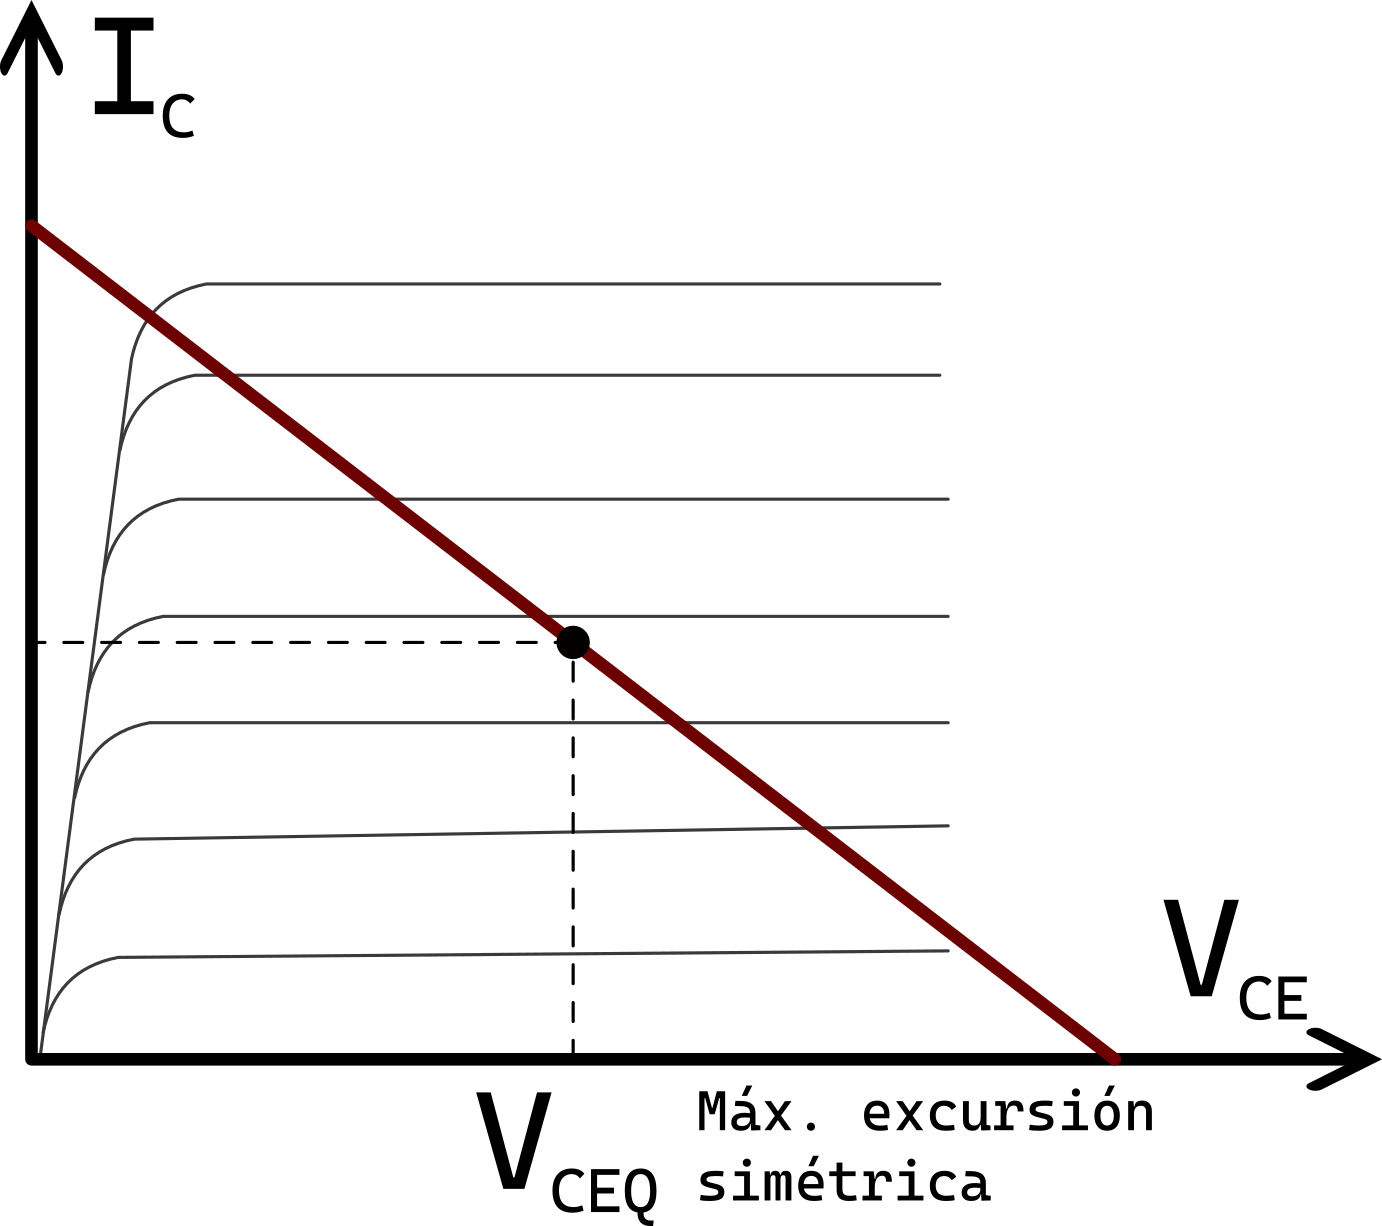
\includegraphics[width = .6 \linewidth]{recta-de-carga}
			
			\subsubtitulo{Aplicación en conmutación}\vspace{-.7cm}
		
			\begin{flushleft}
				Garantizar que: $\beta i_B = 5 i_C$
			\end{flushleft} \vspace{-.2cm}
		
			\begin{tabular}{l l}
				\textsl{Corte} 		& \textsl{Saturación} 				\\[.1cm]
				$i_B = 0$ 			& $v_{CE} = 0.2 V$ 					\\[.1cm]
				Interruptor abierto & Interruptor cerrado
				
			\end{tabular}
		
			\vspace{.2cm}
			
			\subsubtitulo{Aplicación para amplificación}\vspace{-.7cm}
			
			\begin{flushleft}
				\textsl{Máxima excursión simétrica} en
			\end{flushleft}
			
			${v_{CE}}_Q = \dfrac{(v_{CE})_{i_C = 0}}{2}$
			
			\begin{multicols}{2}
				
				\begin{flushleft}
					Polarización por \textsl{resistencia de base}.
				\end{flushleft}
			
				\begin{tabular}{l}
					Varía con $\beta$ \vspace{.1cm}\\
					$V = i_C R_C + v_{CE} +  i_E R_E $ \vspace{.1cm}\\
					$V = i_b R_B + v_{BE} + i_E R_E$
				\end{tabular} 
				
				
				\vspace{1cm}
				
				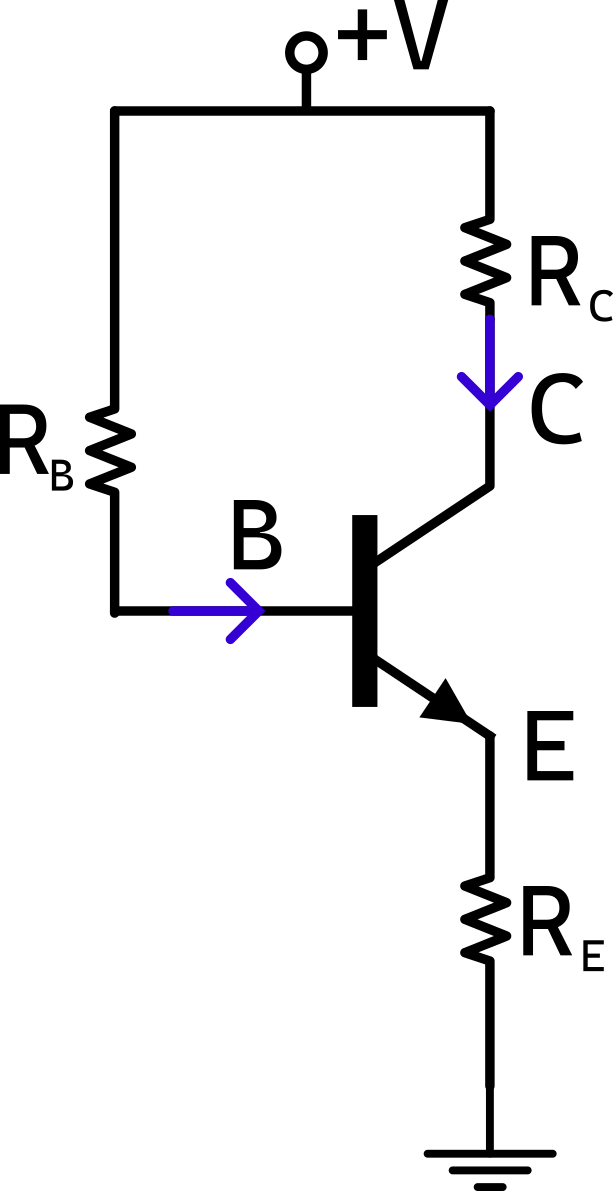
\includegraphics[height = 4cm]{resistencia-de-base}
				
				\columnbreak
				
				\begin{flushleft}
					Polarización por \textsl{divisor de tensión}.
				\end{flushleft}
				
				\begin{tabular}{l}
					No varía con $\beta$ \vspace{.1cm}\\
					$V_{Th} = V_{CC} \dfrac{R_2}{R_2 + R_1}$ \vspace{.1cm} \\
					$R_{Th} = \dfrac{R_1 R_2}{R_1 + R_2}$  \\
				\end{tabular} 
			
				\vspace{.3cm}
				
				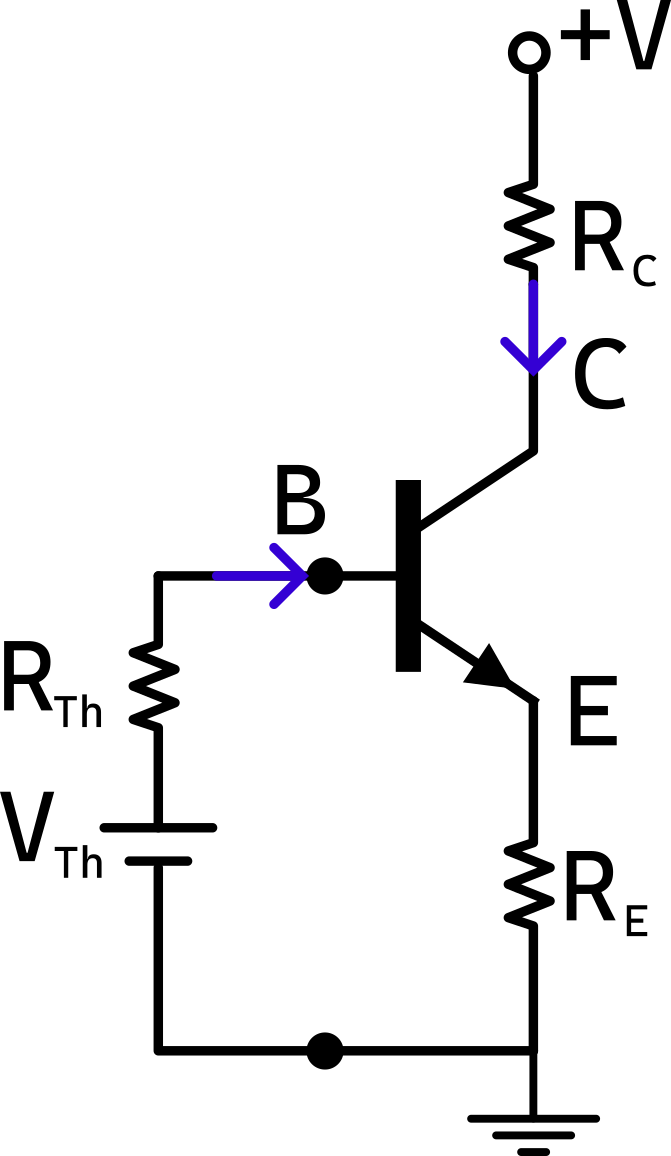
\includegraphics[height = 4cm]{divisor-de-tension}
				
			\end{multicols}
			
			\newpage
			\begin{flushleft}
				Polarización por \textsl{análisis aproximado}.\\[.2cm]
				
				Garantizar que: 	$\beta R_E \geq 10 R_2$
			\end{flushleft}
			
		\end{cajita}

	\end{multicols}
\end{document}